\documentclass[11pt,letterpaper]{article}

%\usepackage{times}
%\usepackage{epsfig}
\usepackage{graphicx}
%\usepackage{amsmath}
%\usepackage{amssymb}
\usepackage{hyperref}
\usepackage{tabularx}
\usepackage[left=1in, right=1in, top=1in, bottom=1in]{geometry}
\usepackage{titling}
\usepackage{setspace}
\usepackage{sectsty}
\usepackage{tabto}
\graphicspath{{./Assignment_02_NOTEBOOK_Geidel_files/}} % adds the assets directory to the path, throw your images there
\usepackage{fancyhdr}
\pagestyle{fancy}
\fancyhf{}
\fancyheadoffset{0cm}
\renewcommand{\headrulewidth}{0pt} 
\renewcommand{\footrulewidth}{0pt}
\fancyhead[R]{\thepage}
\fancypagestyle{plain}{%
  \fancyhf{}%
  \fancyhead[R]{\thepage}%
}

\usepackage{cite}
\usepackage[sectionbib]{natbib}
\renewcommand{\refname}{}

\begin{document}
\fontfamily{ptm}\selectfont
\sectionfont{\fontsize{12}{12}\fontfamily{ptm}\selectfont}
\doublespacing
%%%%%%%%%%%%%%%%%%%%%%%%%%%%%% TITLE %%%%%%%%%%%%%%%%%%%%%%%%%%%%%%%%%%%%%%
\setlength{\droptitle}{1in} 

\title{\large{ASSIGNMENT 2: \\ SALES RECOMMENDATION AGENT \\\vspace{1.2in}}}

\author{
Kevin Geidel \\
MSDS 442: AI Agent Design \& Development \\
Northwestern University \\
May 11, 2025 \\
}

\date{}
\maketitle
\thispagestyle{empty}	
\clearpage
\setcounter{page}{1}

%%%%%%%%%%%%%%%%%%%%%%%%%%%%%% PAGE 1 %%%%%%%%%%%%%%%%%%%%%%%%%%%%%%%%%%%%

\section*{Requirement 1: Graph the Agent with LangChain/LangGraph}
    \tab The construction of the agent and accompanying graph begins in cell 2 (see appendix). 
    The actual assembly of the graph occurs in cell 5. However, some of the components, such as the retriever \textbf{ToolNode} and \textbf{AgentState} class,
    are built above. Following the logic in cell 5 we first instantiate an empty graph:

    \begin{verbatim}
    workflow = StateGraph(AgentState)
    \end{verbatim}

    The \texttt{workflow} object has \texttt{add\_node} and \texttt{add\_edge} methods that allow us to assemble the 
    components created in cells 2-6. The output is displayed graphically in cell 6 (reproduced below.)
    \begin{center}
        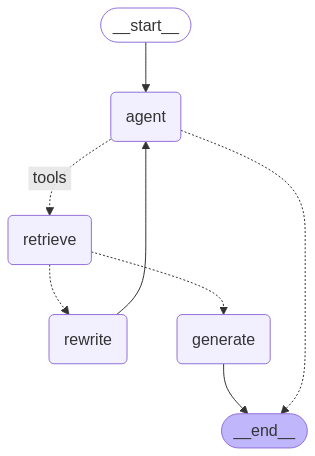
\includegraphics[height=400pt]{Assignment_02_NOTEBOOK_Geidel_5_0.png}
    \end{center}

    \clearpage

\section*{Requirement 2: Load the Dell web pages}
\tab Loading the web pages occurs in in cell 2. A list of URLs are defined and based to the \textbf{WebBaseLoader}.
The \textbf{RecursiveCharacterTextSplitter} chunks the documents into workable pieces. The result is a list of LangChain documents that each have
a portion of each site. The documents are embedded and stored in the ChromaDB vector store.

\section*{Requirement 3: Inspect and comment on four queries}
\tab The first query sent to the agent was \textit{`I want a dell computer for travel that has Intel® Core™ 7 150U.'} The response is reproduced below.
While the response does not mention travel, specifically, it did recommend ultralight designs. Perhaps this was the agent addressing the travel component?
These laptops do have intel 7 processors, so in that sense they are accurate.

\begin{center}
    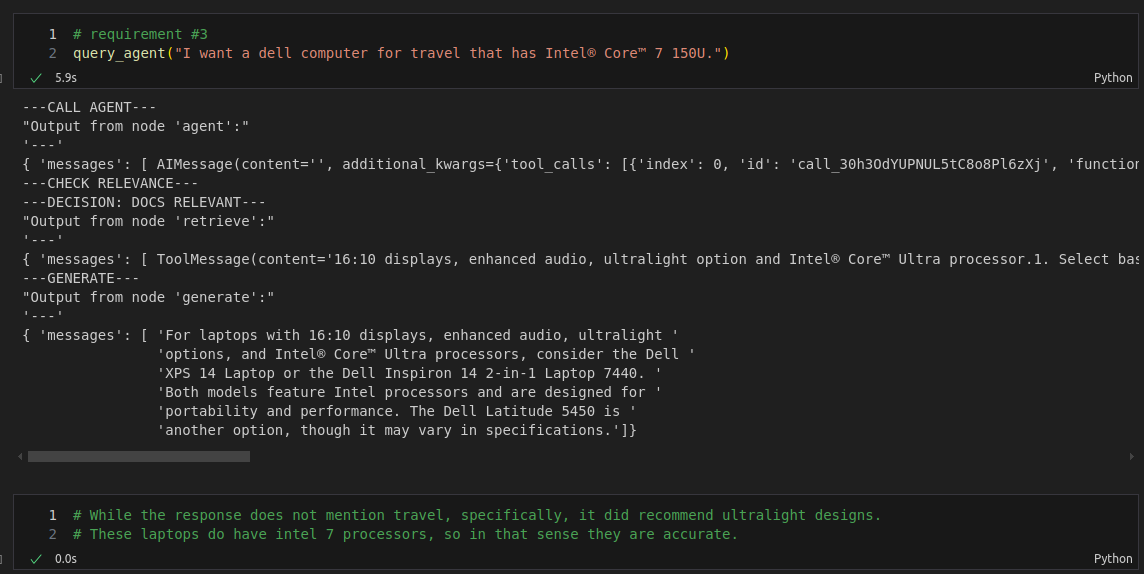
\includegraphics{q1.png}
\end{center}

The second query, displayed below, included specific requirements on the desired memory. The response address this but also includes other options that have different memory specifications. 

\begin{center}
    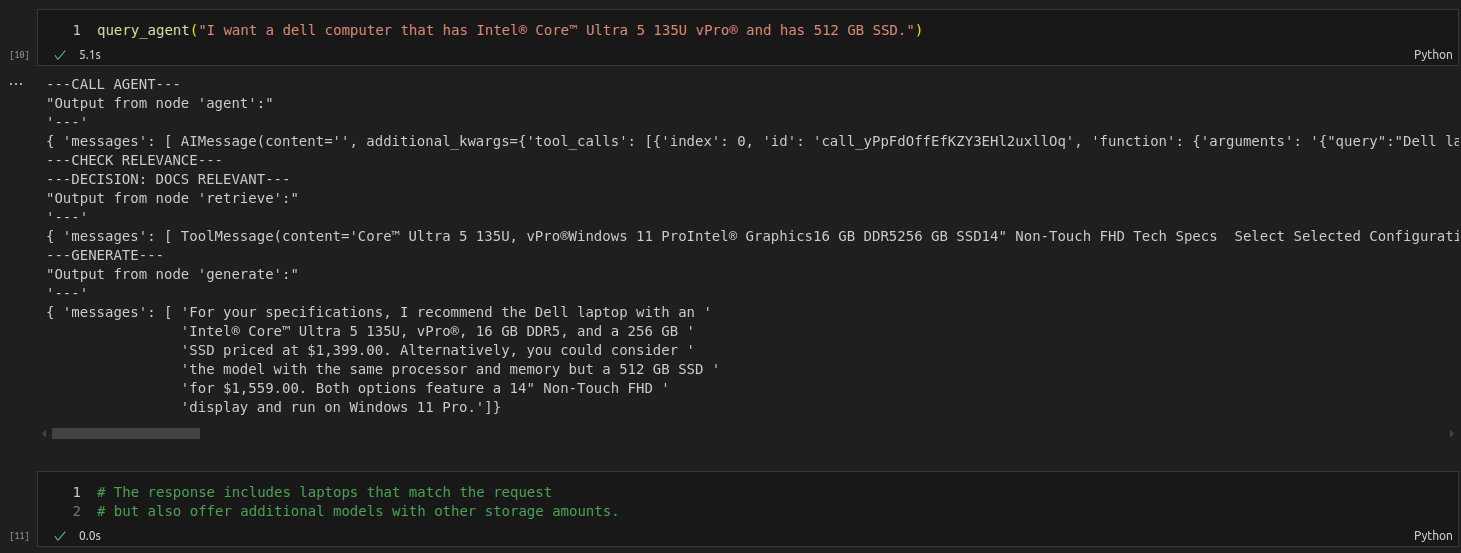
\includegraphics{q2.png}
\end{center}

\begin{center}
    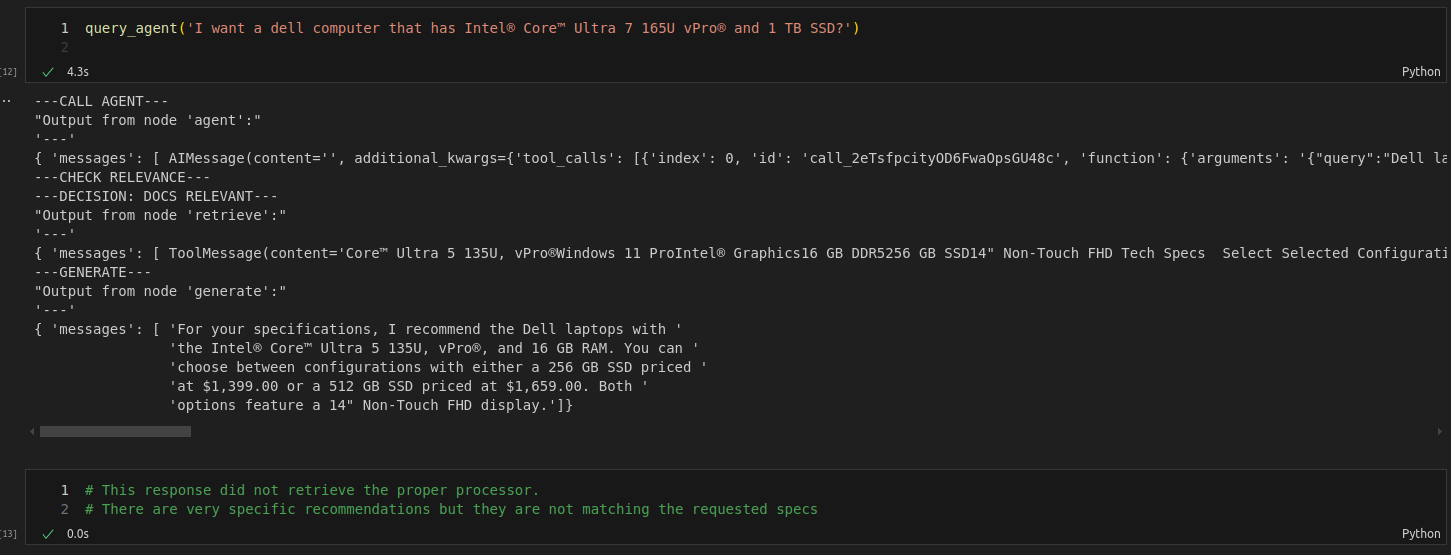
\includegraphics{q3.png}
\end{center}

\begin{center}
    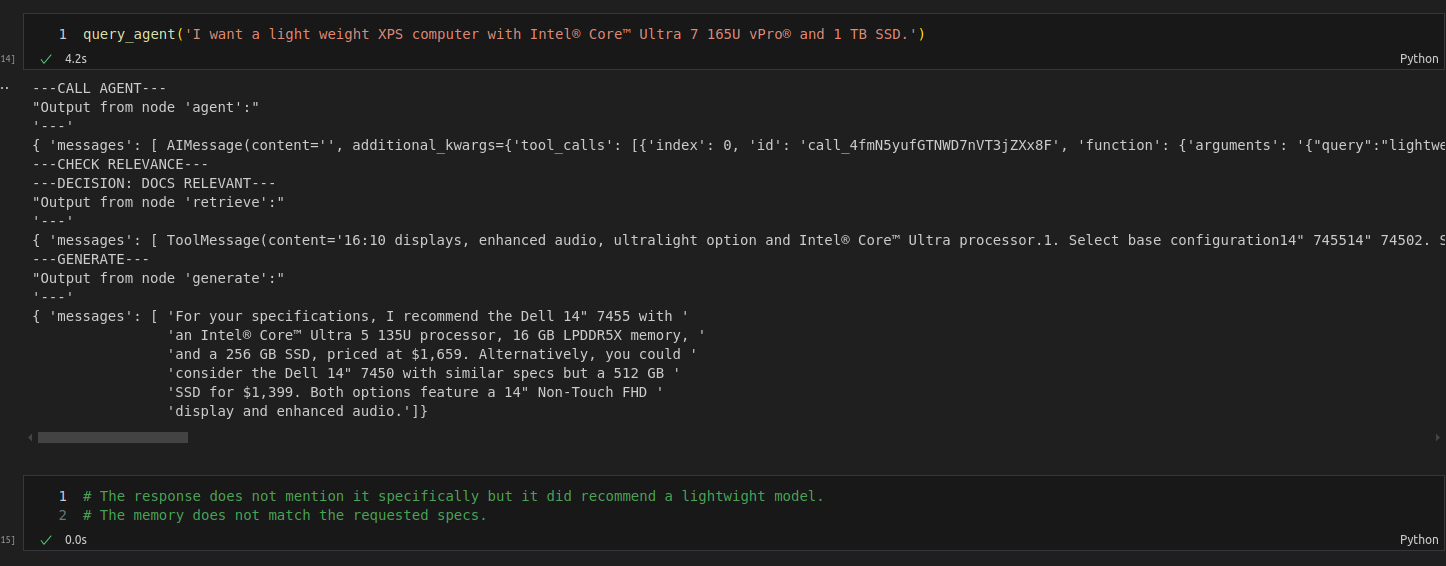
\includegraphics{q4.png}
\end{center}

\begin{center}
    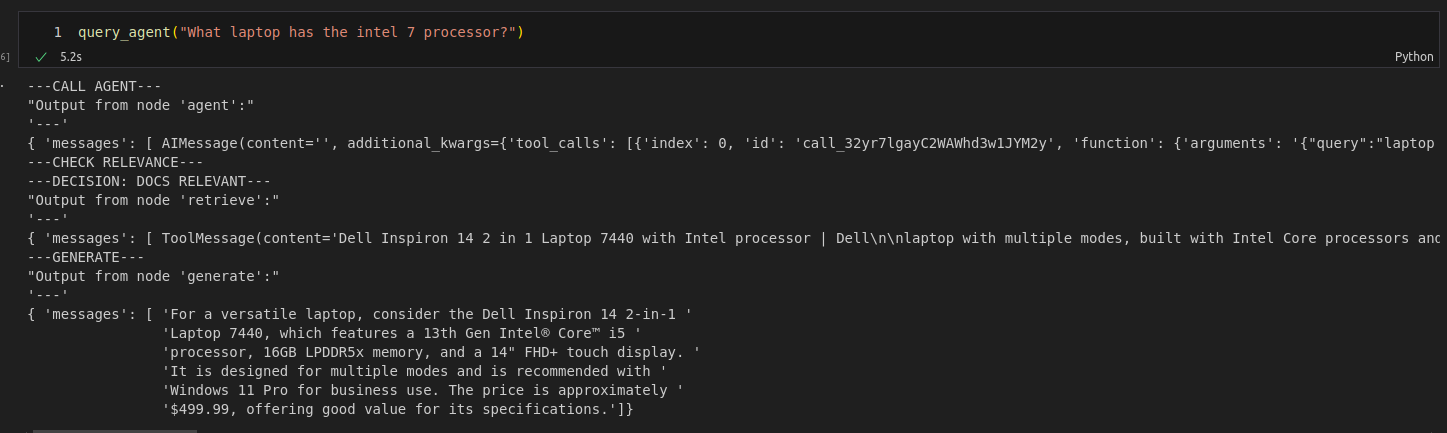
\includegraphics{q5.png}
\end{center}


\section*{Requirement 4: Response consistency}
\tab 

\section*{Requirement 5: Agent improvements}
\tab 


\end{document}